\documentclass[11pt]{article}
\usepackage[margin=1in]{geometry}
\usepackage[T1]{fontenc}
\usepackage{lmodern}
\usepackage{microtype}
\usepackage{graphicx}
\usepackage{booktabs}
\usepackage{array}
\usepackage{hyperref}
\usepackage[numbers,sort&compress]{natbib}
\usepackage{tikz}
\usetikzlibrary{arrows.meta,positioning}
\hypersetup{colorlinks=true,linkcolor=blue,citecolor=blue,urlcolor=blue,
  pdftitle={An Embedded Web-Managed Infrared Learning Remote on the Arduino UNO R4 WiFi},
  pdfauthor={Arijit Kumar Roy},
  pdfsubject={System design and implementation review of an embedded infrared learning remote},
  pdfkeywords={infrared remote control, embedded systems, Arduino, signal capture, reproducibility}}
\title{An Embedded Web-Managed Infrared Learning Remote on the Arduino UNO R4 WiFi: System Design and Implementation Review}
\author{Arijit Kumar Roy\\\small Independent researcher\\\small ORCID: \href{https://orcid.org/0009-0002-5797-8600}{0009-0002-5797-8600}}
\date{November 2026}

\begin{document}
\maketitle

\begin{abstract}
Infrared (IR) remote signals remain a practical interface for consumer devices, yet capturing, organizing, and replaying commands commonly requires dedicated appliances or host-connected tools. This paper describes the design and source-level implementation of IR Learner, an open-source learning remote built around an Arduino UNO R4 WiFi. The system combines interrupt-timed pulse capture, a collection of protocol-specific decoders, hardware-timed carrier generation, persistent command storage, and a browser-accessible HTTP and WebSocket interface. Raw captures are retained as microsecond timing sequences and can be replayed when protocol recognition fails. The repository provides an implementation artifact and a documented hardware configuration; this paper is an engineering description rather than a performance evaluation. We inspect the implementation to distinguish implemented behavior from intended or user-reported behavior. In particular, decoder coverage is uneven, the displayed quality value is heuristic, and the repository does not provide controlled measurements of decoding accuracy, transmission range, timing error, or storage compression. These limitations define a reproducible baseline and a concrete evaluation agenda for future work.
\end{abstract}

\noindent\textbf{Keywords:} infrared remote control; embedded systems; Arduino; signal capture; web interface; reproducible engineering

\section{Introduction}
Infrared remotes encode commands as timed sequences of modulated optical bursts. Learning remotes must capture those sequences, identify their structure where possible, and reproduce them with suitable timing and carrier modulation. A browser-based interface can make these operations accessible without a separate desktop application, but places storage, networking, signal processing, and user interaction on a resource-constrained embedded target.

This report presents IR Learner, a firmware project for the Arduino UNO R4 WiFi. The board pairs a Renesas RA4M1 microcontroller with an ESP32-S3 connectivity module and provides 8~kB of data flash used as EEPROM emulation in the project's storage layer \citep{arduinoUnoR4Datasheet}. The work's contribution is an integrated, inspectable implementation: a pulse-capture and replay path, a small embedded command database, and a local web application. The paper's scope is descriptive. It does not claim measured reliability, broad appliance compatibility, or superiority over established IR libraries. Such claims require controlled tests that are not included in the repository.

\section{System overview}
The firmware is organized around an \texttt{IRManager} coordinator. It initializes persistent storage, the receiver and transmitter, Wi-Fi management, HTTP endpoints, and the embedded web application. Its main loop services these components and handles receiver-state transitions. The browser communicates with the device over HTTP on port~80; WebSocket messages carry live status and logs. The documented hardware uses an HX1838-style demodulating receiver on D2 and an IR emission module on D3. These pin assignments are implementation choices rather than a general hardware requirement.

\begin{figure}[ht]
\centering
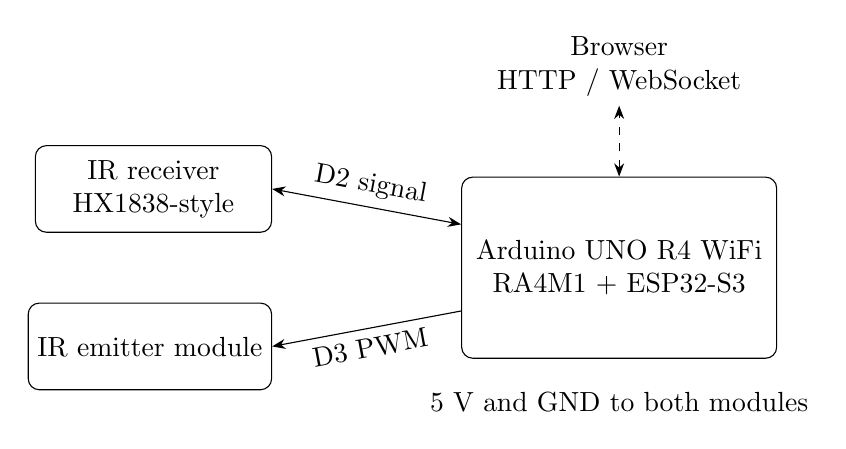
\begin{tikzpicture}[>=Stealth, node distance=1.4cm,
  board/.style={draw, rounded corners, minimum width=4.0cm, minimum height=2.3cm, align=center},
  module/.style={draw, rounded corners, minimum width=3.0cm, minimum height=1.1cm, align=center}]
  \node[board] (uno) {Arduino UNO R4 WiFi\\RA4M1 + ESP32-S3};
  \node[module, left=2.4cm of uno, yshift=1.0cm] (rx) {IR receiver\\HX1838-style};
  \node[module, left=2.4cm of uno, yshift=-1.0cm] (tx) {IR emitter module};
  \draw[<->] (uno.west) ++(0,0.55) -- node[above,sloped] {D2 signal} (rx.east);
  \draw[->] (uno.west) ++(0,-0.55) -- node[below,sloped] {D3 PWM} (tx.east);
  \draw[<->,dashed] (uno.north) -- ++(0,0.9) node[above,align=center] {Browser\\HTTP / WebSocket};
  \node[below=0.3cm of uno] {5 V and GND to both modules};
\end{tikzpicture}
\caption{Documented wiring and communication paths. The emitter is shown as a three-pin module; its internal driver circuitry is not specified by the repository.}
\label{fig:wiring}
\end{figure}

\begin{table}[ht]
\centering
\caption{Principal implementation elements visible in the repository.}
\label{tab:components}
\begin{tabular}{>{\raggedright\arraybackslash}p{0.23\linewidth} >{\raggedright\arraybackslash}p{0.69\linewidth}}
\toprule
Element & Role \\
\midrule
Receiver & Edge-change interrupt on D2; stores up to 400 inter-edge durations in microseconds. \\
Decoder & Attempts protocol-specific timing checks and extracts fields for recognized frames; unmatched captures remain available as raw timings. \\
Transmitter & Uses the Renesas PWM abstraction on D3 to gate an approximately one-third-duty-cycle carrier; provides protocol-specific send methods and raw replay. \\
Storage & Maintains a compact in-memory index and command records in an 8192-byte EEPROM abstraction, including optional raw timing data. \\
Network and UI & Serves an embedded single-page interface, REST-like JSON endpoints, and WebSocket status/log events. \\
\bottomrule
\end{tabular}
\end{table}

\section{Capture and representation}
Learning begins by attaching a change interrupt to D2 and entering a learning state. A falling edge starts capture; subsequent edge intervals are appended to a 400-element \texttt{uint16\_t} buffer. When the line remains without an edge for more than 100~ms, capture is finalized if at least four intervals were recorded. Waiting for a signal is limited to 30~s. Captures exceeding the fixed buffer enter an overflow state. The receiver therefore records the output of a demodulating receiver as alternating edge durations; it does not sample the optical carrier waveform itself.

The decoder applies fixed nominal timing windows, generally with a 30\% tolerance, to the captured intervals. The source includes decoding routines for NEC, Samsung, Sony, Panasonic, LG, JVC, and a heuristic RC5 implementation. The RC6 routine currently returns failure unconditionally, so an RC6-like signal is handled through the raw-capture path rather than decoded into fields. Thus, protocol enumeration and transmitter methods should not be interpreted as evidence that every listed receive decoder is functional.

For a recognized frame, the result contains a protocol identifier, address, command, bit count, and a quality field. The quality field is assigned fixed constants by decoder paths (for example, 95 for several decoders); it is not calculated from repeated samples or a validated error model. The raw fallback exposes the recorded interval array through the API and can be saved and replayed. The web interface sends a nominal 38~kHz carrier for raw signals unless another frequency is supplied.

\section{Transmission, storage, and web interface}
The transmitter gates a PWM output to create carrier marks and disables it for spaces. The default carrier is 38~kHz at approximately 33.3\% duty cycle. The Sony send path selects 40~kHz. Protocol-specific methods construct frames for several named protocols, while \texttt{sendRaw} alternates mark and space durations from a stored array. Actual optical range depends on the emitter circuit, geometry, receiver sensitivity, and ambient conditions and has not been characterized in a controlled setup.

The storage layer reserves regions of an 8~kB EEPROM-compatible address space for configuration, metadata, an offset table, and records. The source defines a maximum of 100 indexed entries, but this is an index limit, not a guarantee that 100 arbitrary raw captures fit in data flash. Raw durations are serialized in 10~microsecond units when their scaled value fits in one byte; larger values use a marker followed by the original 16-bit value. This representation introduces quantization for the one-byte case. While the project README describes the scheme as run-length compression and reports an approximate reduction, source inspection shows per-duration scaling/escape serialization rather than run-length encoding. No representative corpus or measured compression ratio is supplied.

The embedded interface provides operations to inspect status and stored codes, start and stop learning, transmit or delete/rename commands, and import or export database JSON. Wi-Fi can join configured infrastructure or fall back to a local access point after connection failure; mDNS is available in connected mode. The firmware exposes unauthenticated local-network endpoints, so the intended deployment context is a trusted LAN. The checked-in example configuration is deliberately not reproduced in this paper.

\section{Implementation review and limitations}
The following are source-level observations, not measured outcomes:
\begin{itemize}
  \item \textbf{Uneven decoder maturity.} Several decoders use frame lengths and fixed timing windows; RC5 uses a simplified transition heuristic, and RC6 decoding is not implemented. Repeat frames and protocol variants may not match these assumptions.
  \item \textbf{Unvalidated quality indicator.} Values assigned to the quality field are constants associated with code paths, not empirical probabilities or calibrated quality estimates.
  \item \textbf{Unmeasured performance.} The repository does not include a labeled remote corpus, capture-success trials, false-decode rates, replay timing measurements, or repeatable range tests. The status endpoint's flash-usage value is a hard-coded estimate, not a runtime measurement.
  \item \textbf{Finite capture and storage.} The receiver buffer caps a frame at 400 intervals. Available nonvolatile space is shared by settings, metadata, and signal records; record capacity therefore depends on each command's representation.
  \item \textbf{Security boundary.} The web service has no authentication or transport encryption. Its APIs should remain confined to a trusted local network and should not be exposed directly to the public internet.
\end{itemize}

These constraints suggest a future evaluation that compares captures against a documented reference set across multiple repetitions and orientations; reports protocol-wise precision, recall, and raw replay success; measures timing and carrier frequency with suitable instrumentation; profiles actual flash and SRAM use; and quantifies storage size and reconstruction error. The protocol implementations should also be checked against primary protocol specifications or a mature reference implementation such as Arduino-IRremote, which documents broad protocol coverage and support for Renesas-based boards \citep{arduinoIRremote}.

\section{Reproducibility and artifact availability}
The firmware source inspected for this report is pinned to Git commit \texttt{8baa14c} \citep{irLearnerRepo}; the bibliography records its full hash, which identifies the firmware baseline discussed here. The paper source is maintained separately in the working tree and should be included in the next tagged release or Zenodo archive. The repository identifies Arduino UNO R4 WiFi as the target and documents the D2 receiver and D3 emitter wiring. The paper can be rebuilt with a LaTeX distribution and BibTeX by running \texttt{pdflatex IR\_Learner\_paper.tex}, \texttt{bibtex IR\_Learner\_paper}, followed by two further \texttt{pdflatex} passes. No device measurements are required to reproduce this source-level report. The project source prepared for deposit is licensed under the MIT License. For a Zenodo release, the deposited source and PDF should be versioned together with a repository snapshot; the DOI should be added after Zenodo assigns it.

\section{Conclusion}
IR Learner demonstrates an integrated architecture for learning and replaying infrared commands through a local browser interface on a compact microcontroller platform. Its distinguishing system-level feature is the coupling of raw timing capture and replay with protocol-oriented control, local persistence, and a web API. The current artifact is best regarded as a functional prototype and a basis for experimental work. Reliable claims about compatibility, accuracy, storage efficiency, or range await systematic measurements, and the source should be treated as the definitive description of implemented behavior.

\bibliographystyle{unsrtnat}
\bibliography{IR_Learner_paper}
\end{document}
